Oral anticoagulation has been shown to prevent thrombembolism efficiently for several indications.  However the precondition is that the inhibition of clotting, measured by \ac{INR}, is between close borders. To weak inhibition is associated with the risk of thrombembolic events, to strong inhibition increases the risk of gastrointestinal or cerebral bleedings \cite{Van_der_Meer_1993}.

Measurement of INR at fixed intervals and calculating the time in therapeutic range is necessary to protect patients under therapy with \ac{VKA} from complications.

In studies and daily clinical work \ac{TTR} is be calculated by different methods \cite{Kaatz_2008}:


The simplest method calculates the percentage of \ac{INR} within the therapeutic range \ac{PINRR}. The \ac{PINRR} method counts how many measurements had INR results in range. This number is divided by the total numbers of visits. For the data of patient depicted in figure \ref{example_patient} 18 of 26 values are in range. So the estimation for time in therapeutic range is $\frac{18}{26}= 69 \%$. 

\begin{tabular}{l*{8}{c}}
	tp& 
	0 & 3 & 6.7 & 10.7 & 15.7 & 19.7 & 24.7 & 29 \\
	inr&
	\colorbox{green}{2.37}&
	\colorbox{green}{2.41}&
	\colorbox{green}{2.47}&
	\colorbox{green}{2.41}&
	\colorbox{green}{2.76}&
	\colorbox{green}{2.70}&
	\colorbox{green}{2.93}&
	\colorbox{green}{2.75}\\
	tp&
	32 & 37 & 42.7 & 48.9 & 51 & 55 & 57 & 58 \\
	inr&
	\colorbox{green}{2.79}&
	\colorbox{green}{2.58}&
	\colorbox{green}{2.76}&
	\colorbox{red}{1.89}&
	\colorbox{green}{2.16}&
	\colorbox{red}{3.56}&
	\colorbox{red}{4.45}&
	\colorbox{red}{3.21} \\
	tp&
	111.1&112.9&116.9&120.9&124.9&127.9&131.9&135.9 \\
	inr&
	\colorbox{red}{3.85}&
	\colorbox{red}{3.89}&
	\colorbox{red}{3.28}&
	\colorbox{red}{4.10}&
	\colorbox{green}{2.28}&
	\colorbox{green}{2.21}&
	\colorbox{green}{2.72}&
	\colorbox{green}{2.35} \\
	tp&
	139.3 & 141.9\\
	inr&
	\colorbox{green}{2.67}&
	\colorbox{green}{2.27}
	
\end{tabular}


\begin{figure}
	\centering
	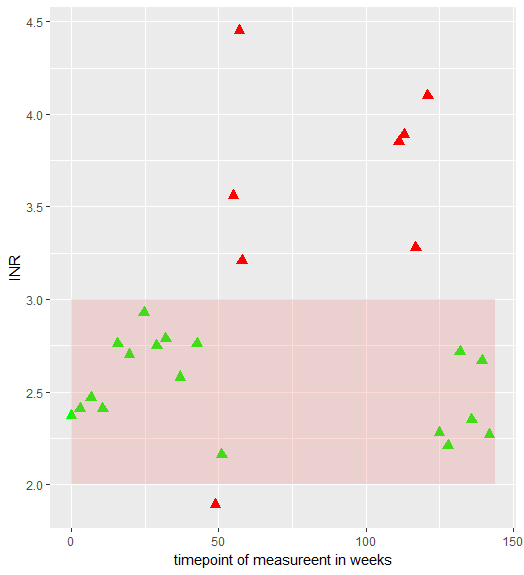
\includegraphics{inr_scatterplot.png}
	\label{example_patient}
	\caption{INR values over time of a single example patient. Green points are values in range, red points values out of range} 
\end{figure}

The more complex method of calculation \ac{TTR} is the so called "Rosendaal method" \cite{Rosendaal_1993}. It has become the mostly used method of determing how well a patient is maintaining his \ac{INR} test results in clinical studies. This method measures percantage time in\ac{TTR} using linear interpolation. The underlying assumption is that the \ac{INR} value between two measurements vary in a linear manner from the first to second value. 

One possibility to calculate \ac{TTR} is to divide the time between two measurements in  halves and allocate the first halve to the first \ac{INR} and second halve to second \ac{INR}.

The more distinguished possibility assumes that changes between consecutive \ac{INR} are linear over time and takes account of the steepness of change of inr-values between measurements. Calculating \ac{TTR} by "Rosendaal-Method" is more difficult when one measurement is within the therapeutic range and the second is out. The part of time in \ac{TTR} is the calculated by

\begin{align}
	\frac{\text{difference of inr in range}}{\text{difference of inr}} * {\text{difference of time}}
\end{align} 

For example at timepoint 51 the inr value is 2.16 in range. At the next timepoint 55 the inr value is 3.56 out of therapeutic range. 
The part of time in therapeutic range between the two measurements is calculated by

\begin{align} 
\text{time in therapeutic range} = \frac{3-2.16}{3.56-2.16}*(55-51)=\frac{0.84}{1.4}*4=3
\end{align}. 

So it is assumed that 3 weeks of the 5 weeks between the two measurements the \ac{INR} was in therapeutic range an two weeks out of it. 

Calculating the \ac{TTR} for the example patient shows, that the \ac{INR} was 83.5\% of time in therapeutic range.   
     
One problem with the Rosendaal linear extrapolation method is that it is unknown whether the \ac{INR} really varies linear between measurements. The linear model is a simplification because the real shape of the \ac{INR} course is unknown. But linear interpolation may not account for dose changes that are not followed shortly thereafter by repeat \ac{INR} testing (figure \ref{rosendaal_examples}).

\begin{figure}
	\centering
	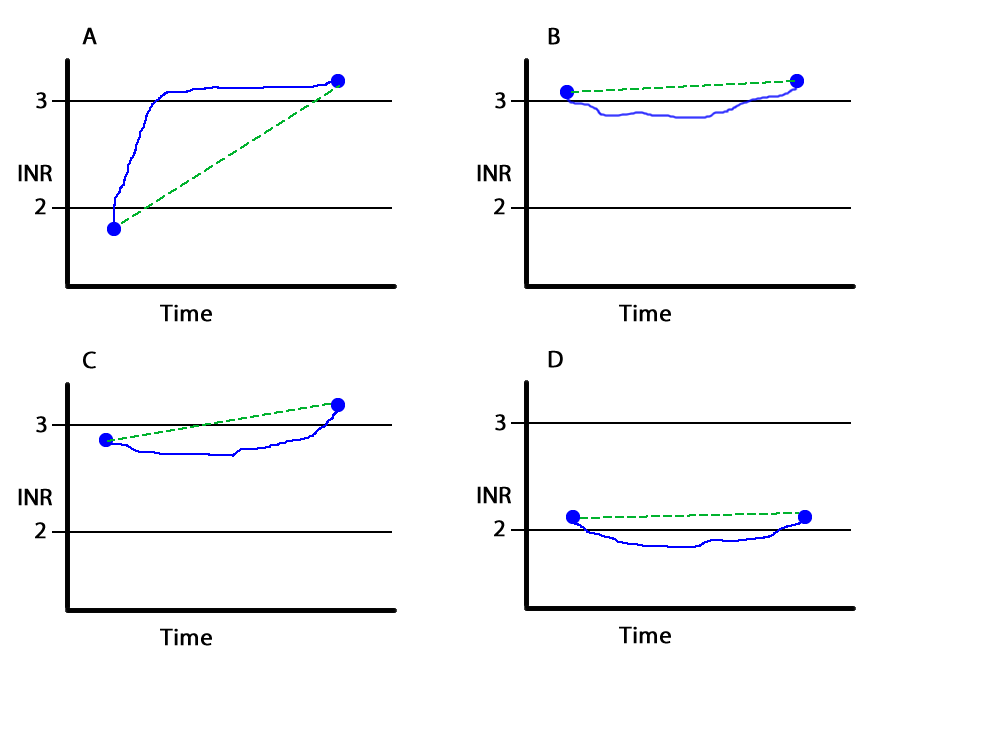
\includegraphics{rosendaal_examples.png}
	\label{rosendaal_examples}
	\caption{Examples of misevaluation  of \ac{INR} course (blue line) by linear interpolation (dotted line) between \ac{INR} measurements (blue points) 
	A: Both \ac{INR} values are out of range. The INR raises fast, but the lineaar interpolation overestimates \ac{TTR}. B: Both \ac{INR} measurements are hardly out of range, but the \ac{INR} course is in range. The \ac{TTR} is underestimated. C: One \ac{INR} is in range, the second out. The \ac{INR} course is in range most of the time. The \ac{TTR} is underestimated by linear interpolation. D: Both \ac{INR} values are in range. The \ac{INR} course is under the range most of the time. The \ac{TTR} is overestimated by linear interpolation.}
\end{figure}

